As a systems research project, the focus of this study revolves around software and in particular, developing more efficient data-intensive computing pipelines that find wide application in machine learning and training of neural networks. Software, according to the Green Software Foundation \cite{GreenSoftwareFoundation}, can be "part of the climate problem or part of the climate solution" \cite{WhatGreenSoftware2021}. We can define Green Software as a software that reduces its impact on the environment by using less physical resources, and less energy and optimizing energy use to use lower-carbon sources \cite{WhatGreenSoftware2021}. In the context of \gls{ML} and training of neural networks, reducing training time (and so also the read and write latency operation on the dataset) has been proven to positively impact the reduction in carbon emissions \cite{pattersonCarbonEmissionsLarge2021,pattersonCarbonFootprintMachine2022}.

This project, by aiming to reduce the latency (seconds) and thus increase the data throughput (rows/second) for reading and writing on Delta Lake tables on \gls{HopsFS}, follows the key green software principles reducing \gls{CPU} time use compared to the previous pipeline. This leads to a lower carbon footprint, as less energy is being used.

This project contributes to the \glspl{SDG} 7 (Affordable and Clean Energy) and 9 (Industry Innovation and Infrastructure) \cite{SustainableDevelopment}, more specifically the targets 7.3 (Double the improvement in energy efficiency) and 9.4 (Upgrade all industries and infrastructures for sustainability). This work achieves this by reducing the read and write latency of data on Delta Lake tables, and thus increasing the data throughput. This means that the same amount of data can be read or written in a smaller amount of time, reducing the use of resources (\gls{CPU} or \gls{GPU} computing time), thus reducing energy usage. This decrease in energy consumption will lead to a smaller carbon footprint (if the same amount of data is read or written). 

\begin{figure}
    \centering
    \begin{subfigure}[b]{0.5\linewidth}
        \centering
        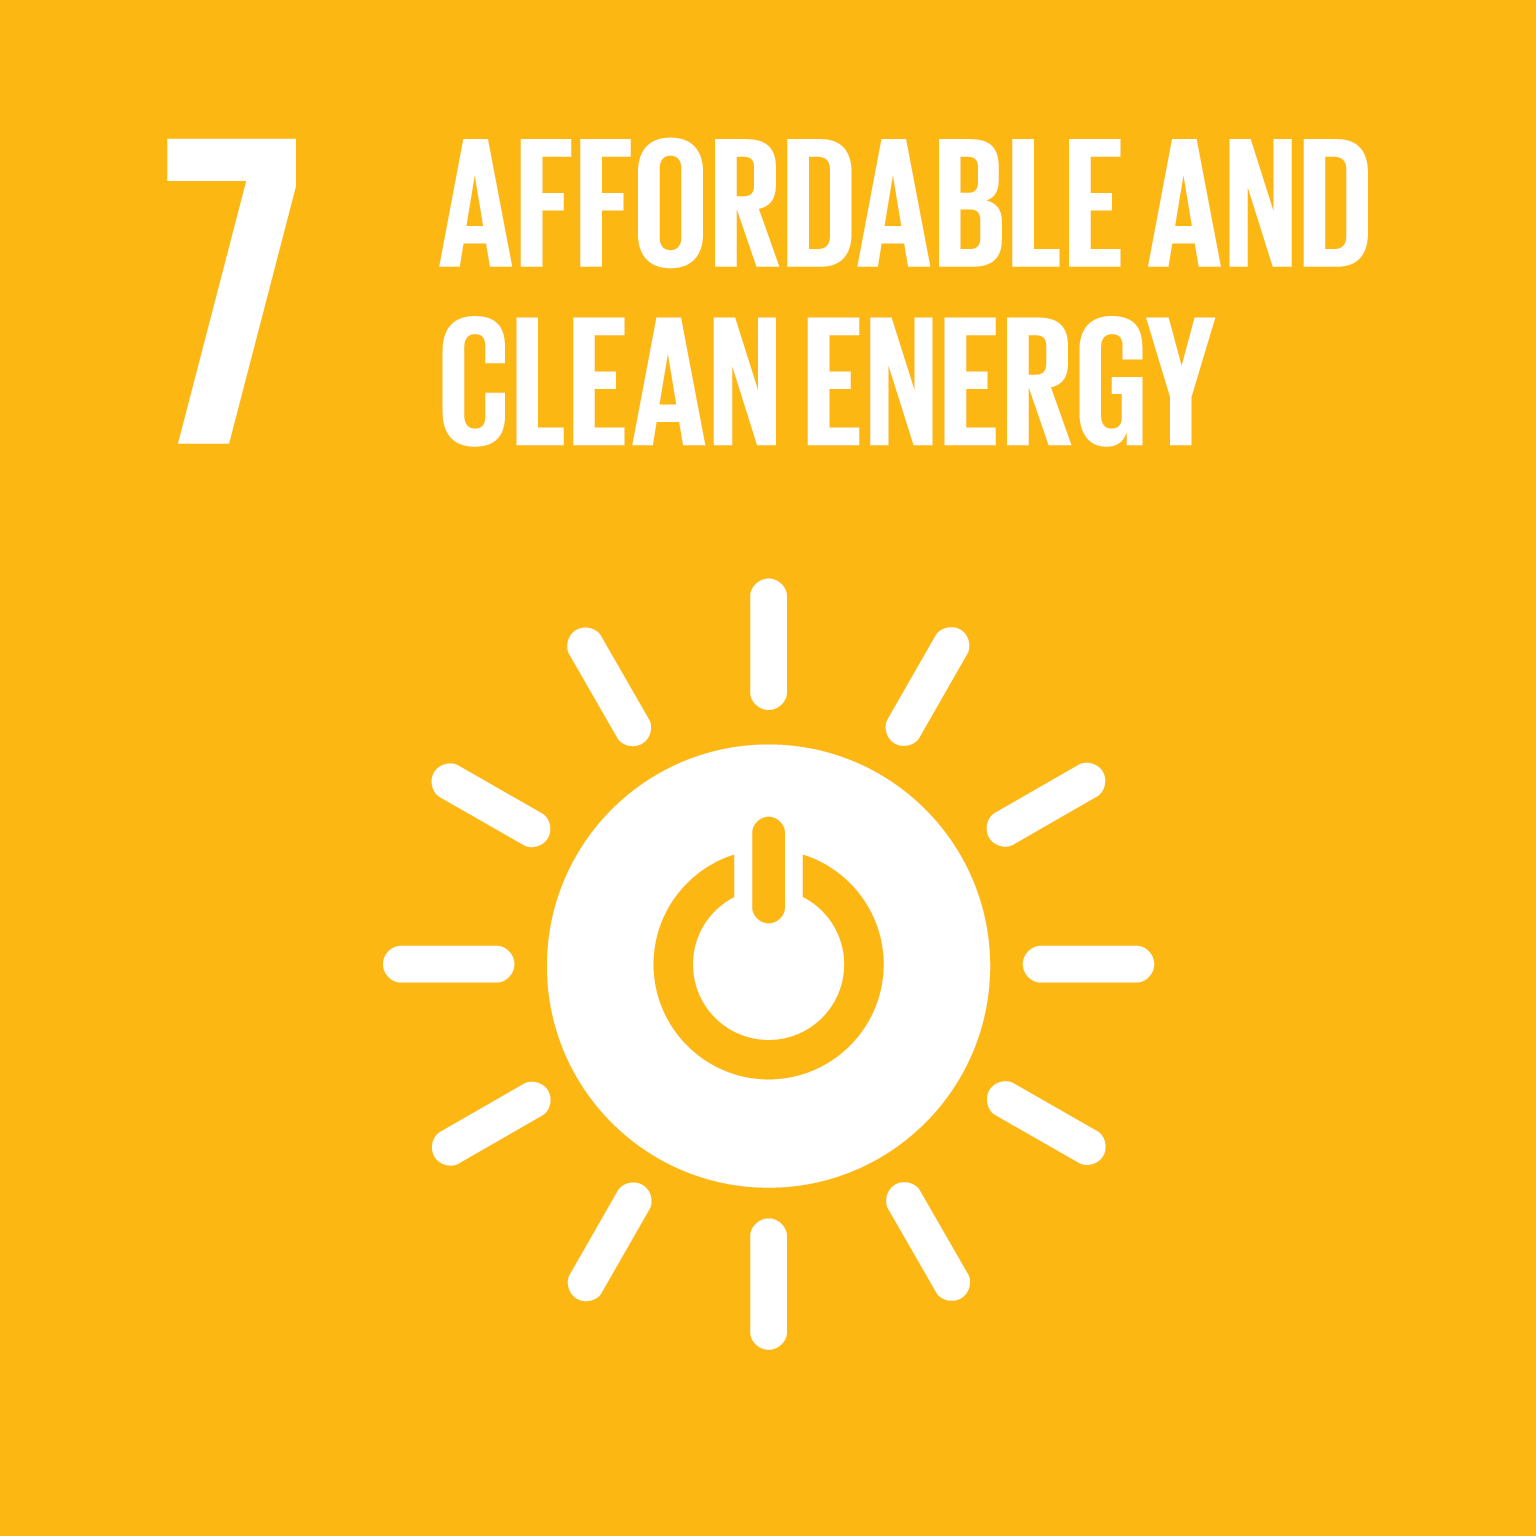
\includegraphics[width=0.6\linewidth]{figures/1-introduction/E_SDG_goals_icons-07.png} 
        \label{fig:sdg07}
    \end{subfigure}\hfill
    \begin{subfigure}[b]{0.5\linewidth}
        \centering
        
\includegraphics[width=0.6\linewidth]{figures/1-introduction/E_SDG-goals_icons-09.png}
        \label{fig:sdg09}
	\end{subfigure}
	\caption{\glstext{SDG} supported by this thesis}
	\label{fig:sdgs}
\end{figure}

Ultimately, this leads to an improvement in energy efficiency and a reduction in the carbon footprint of the data-intensive computing pipelines that find wide application in machine learning and training of neural networks.
